\documentclass[12pt]{beamer}
\usetheme{PaloAlto}
\usepackage[utf8]{inputenc}
\usepackage{amsmath}
\usepackage{amsfonts}
\usepackage{amssymb}
\usepackage{graphicx}
\usepackage{hyperref}
\author[Daniel Pabón\\ Sergio Bolivar]{Daniel Ernesto Pabón Moreno\\ \url{dpabonw@gmail.com}\\
Sergio Andres Bolivar Santamaria\\
\url{sergio.bolivar@hotmail.com}\\
Estudiantes de Biología\\
}
\title{Introducción a R}
\setbeamercovered{transparent} 
%\setbeamertemplate{navigation symbols}{} 
\logo{
\includegraphics[scale=0.17]{images/Rlogo}} 
\institute{\href{https://pasoeco.co/}{Grupo de Estudios en Paisajes Socio Ecológicos}\\
Universidad Industrial de Santander} 
\date{16-01-2017} 

\begin{document}
\begin{frame}
\titlepage
\end{frame}
\section{¿Qué es R?}
\begin{frame}{¿Qué es R?}
\begin{enumerate}[<+->]
\item ¿Programa?
\item ¿Lenguaje de Programación?
\item ¿Herramienta Estadística?
\end{enumerate}
\begin{center}
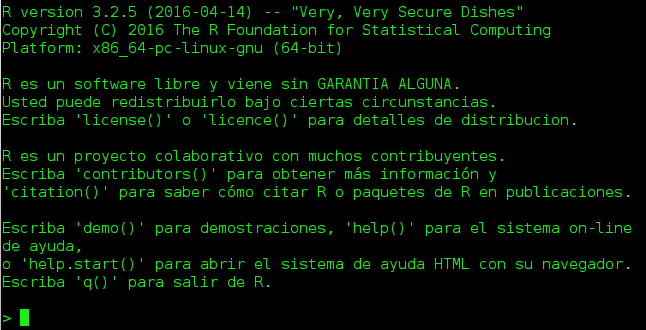
\includegraphics[scale=0.5]{images/image1}
\end{center}
\end{frame}
\section{Powered By}
\begin{frame}{Powered By:}
\begin{center}
\framesubtitle{GNU-FSF}
\href{https://www.gnu.org/}{
\includegraphics[scale=0.15]{images/gnu}}
\end{center}
\end{frame}
\section{Descargar}
\begin{frame}{¿Dónde lo puedo conseguir?}
\framesubtitle{\url{https://www.r-project.org/}}
\begin{center}
\href{https://www.r-project.org/}{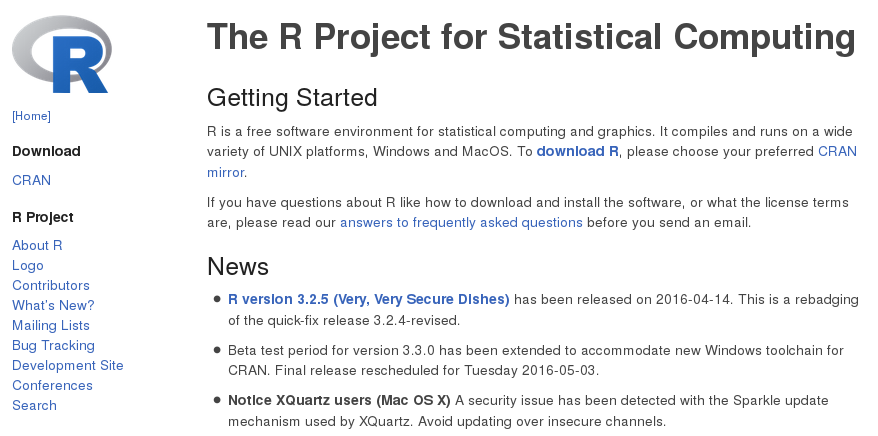
\includegraphics[scale=0.44]{images/image2}}
\end{center}
\end{frame}
\section{Paquetes}
\begin{frame}{CRAN}
\framesubtitle{Comprehensive R Archive Network}
\begin{center}
\textbf{\emph{¡¡9896!!}}
\
\
\href{https://cran.r-project.org/web/packages/available_packages_by_name.html}{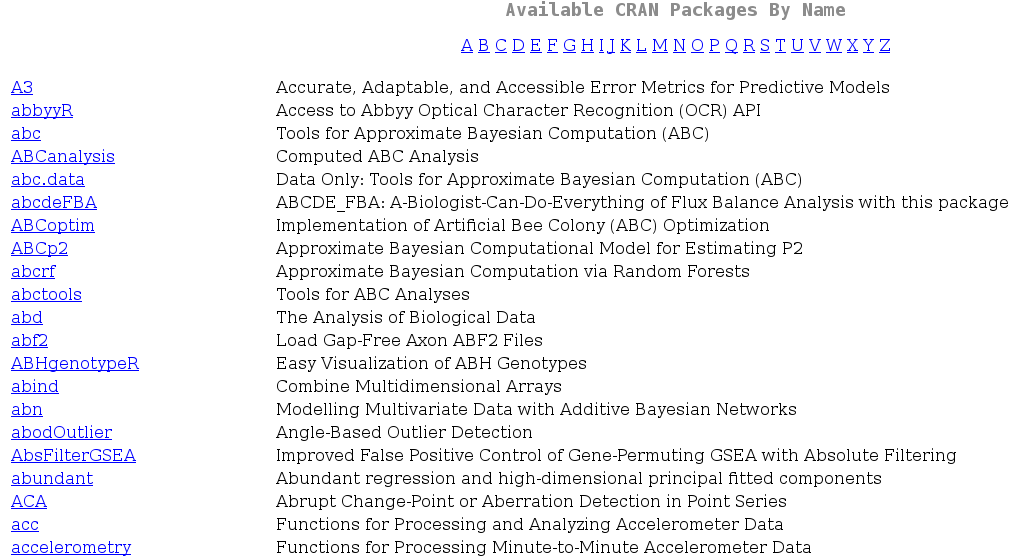
\includegraphics[scale=0.3]{images/image3}}
\end{center}
\end{frame}

\begin{frame}{Bioconductor}
\framesubtitle{\url{http://www.bioconductor.org/}}
\begin{center}
\href{http://www.bioconductor.org/}{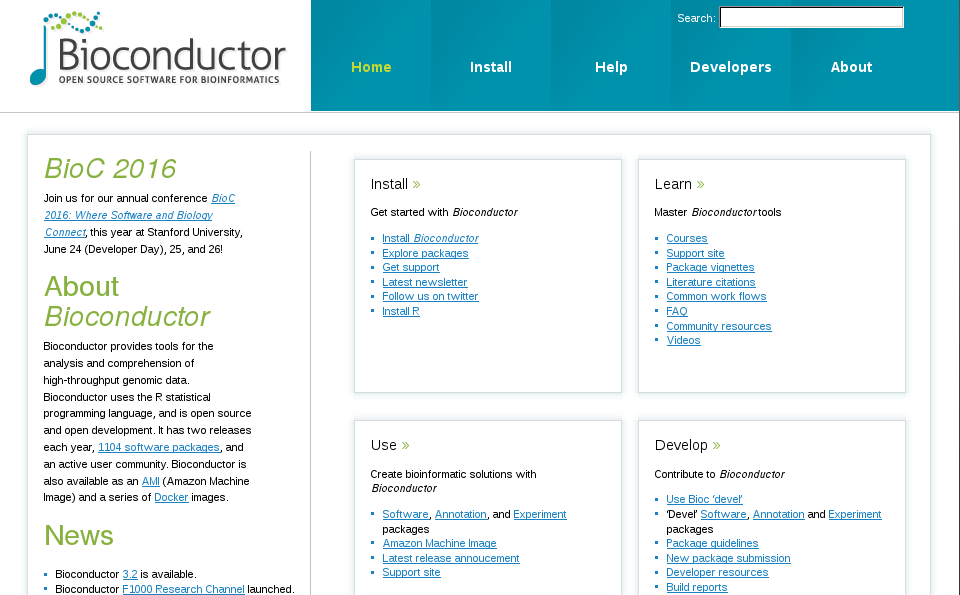
\includegraphics[scale=0.35]{images/image4}}
\end{center}
\end{frame}
\section{¿Dónde puedo aprender?}
\begin{frame}{¿Dónde puedo aprender?}
\begin{enumerate}[<+->]
\item \href{https://www.codeschool.com/courses/try-r}{Code School}
\item \href{https://www.coursera.org/courses?languages=en&query=r}{Coursera}
\item \href{https://www.udemy.com/courses/search/?ref=home&src=ukw&q=R&lang=en}{Udemy}
\item \href{https://archive.org/details/TheRBook}{The R Book}
\item \href{https://cran.r-project.org/doc/contrib/Short-refcard.pdf}{R refcard}
\item \href{http://www.statmethods.net/}{Quick-R}
\item \href{https://cran.r-project.org/doc/contrib/rdebuts_es.pdf}{R para principiantes}
\item \href{http://swirlstats.com/}{Swirl}
\end{enumerate}    
\end{frame}

\section{IDE}
\begin{frame}{IDE}
\framesubtitle{Integrated Development Environment
}
\begin{enumerate}[<+->]
\item \href{http://www.rcommander.com/}{R Commander}
\item \href{https://www.rstudio.com/}{R Studio}
\item \href{http://ess.r-project.org/}{ESS}
\end{enumerate}
\end{frame}
\section{Rstudio}
\begin{frame}{Rstudio}
\framesubtitle{\url{https://www.rstudio.com/}}
\begin{center}
\href{https://www.rstudio.com/}{
\includegraphics[scale=0.35]{images/image5}}
\end{center}
\end{frame}

\begin{frame}{Rstudio}
\framesubtitle{Estructura}
\begin{center}
\includegraphics[scale=0.32]{images/rstudio}
\end{center}
\end{frame}
\begin{frame}{Rstudio}
\framesubtitle{Estructura}
\begin{center}
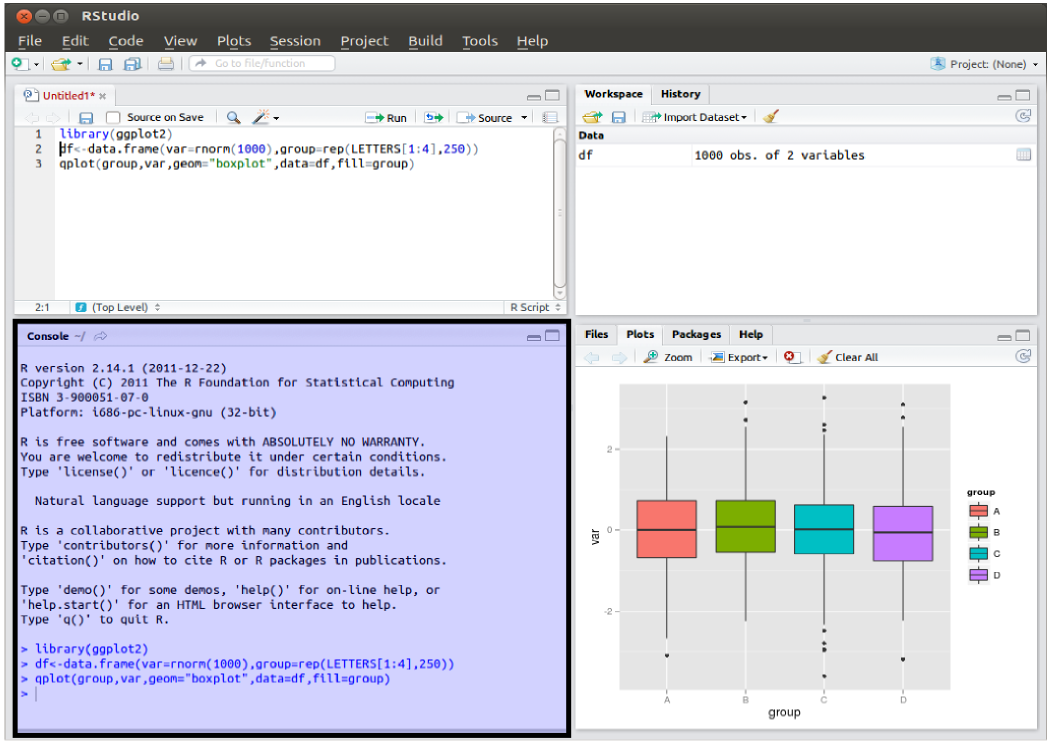
\includegraphics[scale=0.32]{images/rstudio1}\\
\footnotesize{Ventana de Consola}
\end{center}
\end{frame}

\begin{frame}{Rstudio}
\framesubtitle{Estructura}
\begin{center}
\includegraphics[scale=0.32]{images/rstudio2}\\
\footnotesize{Ventana de Edición (Script)}
\end{center}
\end{frame}

\begin{frame}{Rstudio}
\framesubtitle{Estructura}
\begin{center}
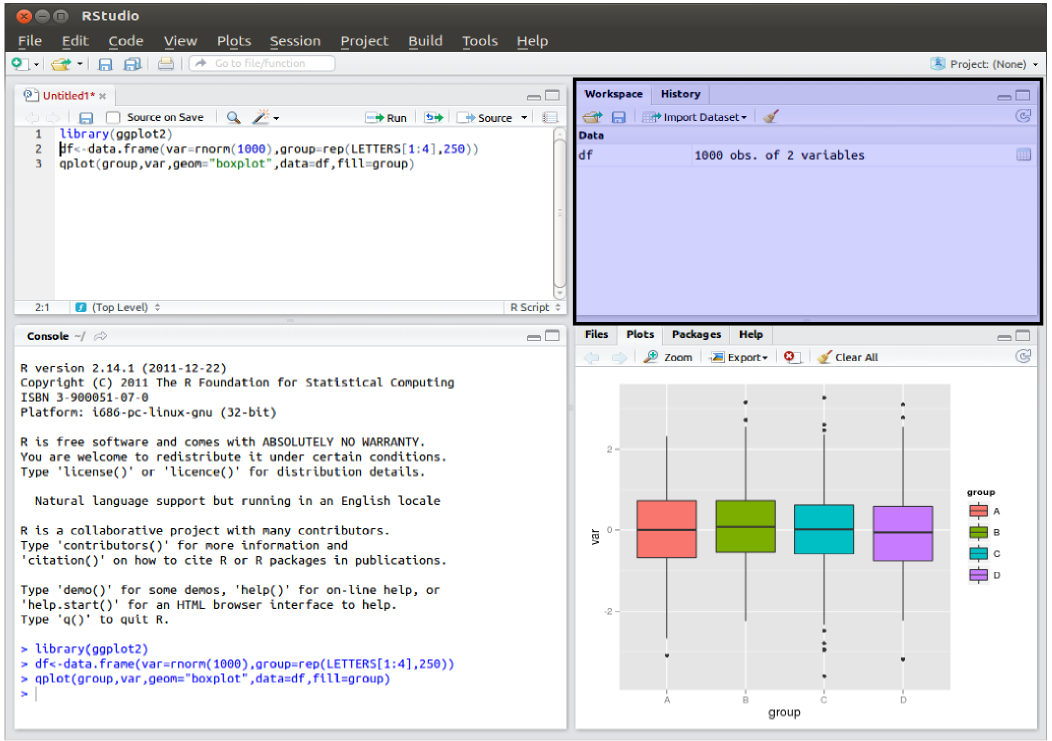
\includegraphics[scale=0.32]{images/rstudio3}\\
\footnotesize{Ventana de Historial}
\end{center}
\end{frame}

\begin{frame}{Rstudio}
\framesubtitle{Estructura}
\begin{center}
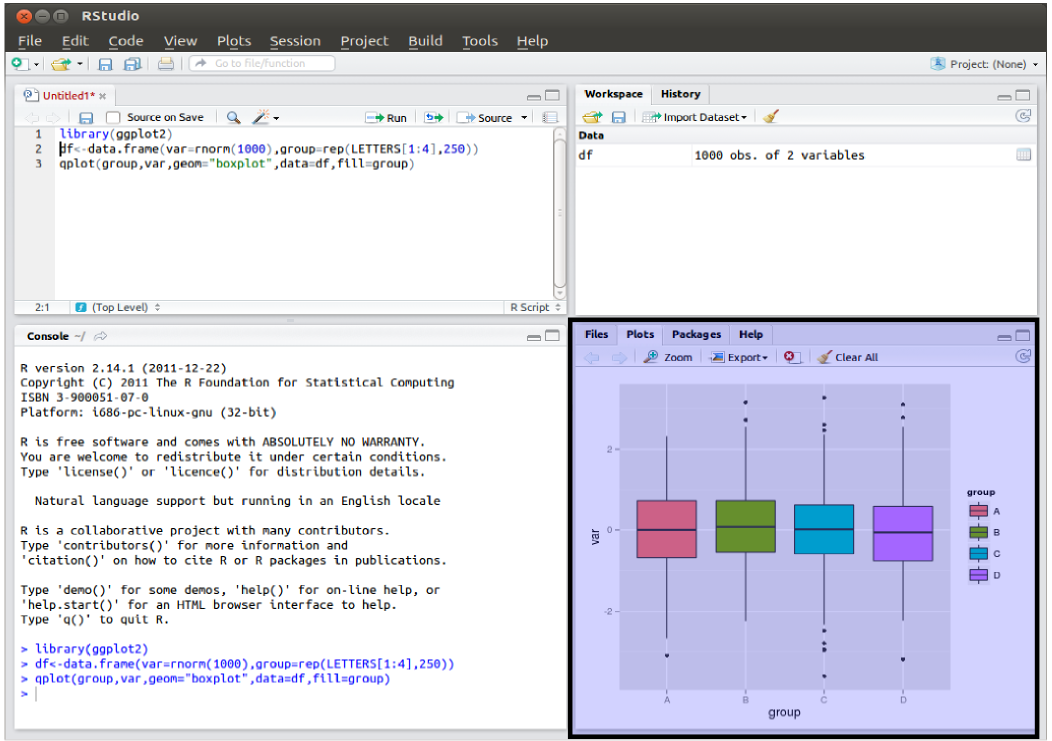
\includegraphics[scale=0.32]{images/rstudio4}\\
\footnotesize{Miscelanea}
\end{center}
\end{frame}


\begin{frame}
\begin{center}
\begin{LARGE}
Slides powered by\\
\href{https://latex-project.org/intro.html}{\LaTeX}
\end{LARGE}\\
\end{center}
\begin{center}
\href{https://github.com/dpabon/R_introduction}{Github}\\
\end{center}
\begin{center}

\includegraphics[scale=0.4]{images/cc}
\end{center}
\end{frame}
\end{document}